\clearpage
\section{Diffusion Distance}

The diffusion distance is given by $\sqrt{Dt}$, which is found in the equation that is used to describe the concentration after a time $t$ in a thin layer of the diffusing species is concentrated at $x=0$ of a semi-infinte sample \cite{diff}:
\begin{align}
  \label{eq:3}
  c(x,t)&=\dfrac{M}{\sqrt{\pi D t}exp\left(-\dfrac{x^2}{4DT}\right)}
\end{align}

\begin{figure}[h]
 \centering
 \captionsetup{justification=centering}
  \subfloat[]{
   \label{fig:d}
    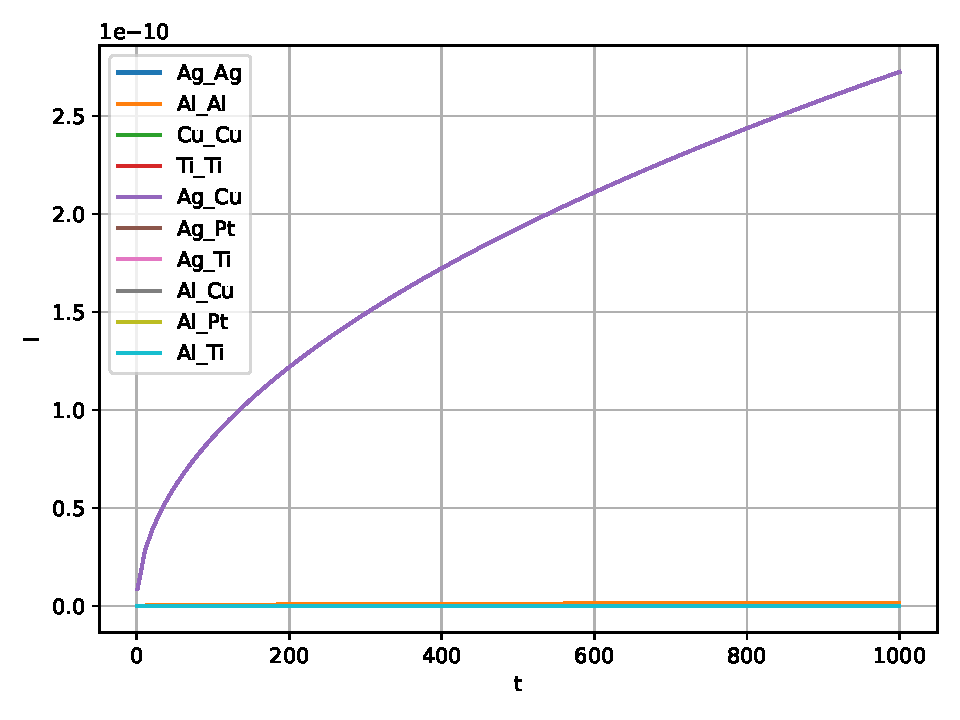
\includegraphics[width=0.5\textwidth]{graficas/l.pdf}}
  \subfloat[]{
   \label{fig:lnd}
    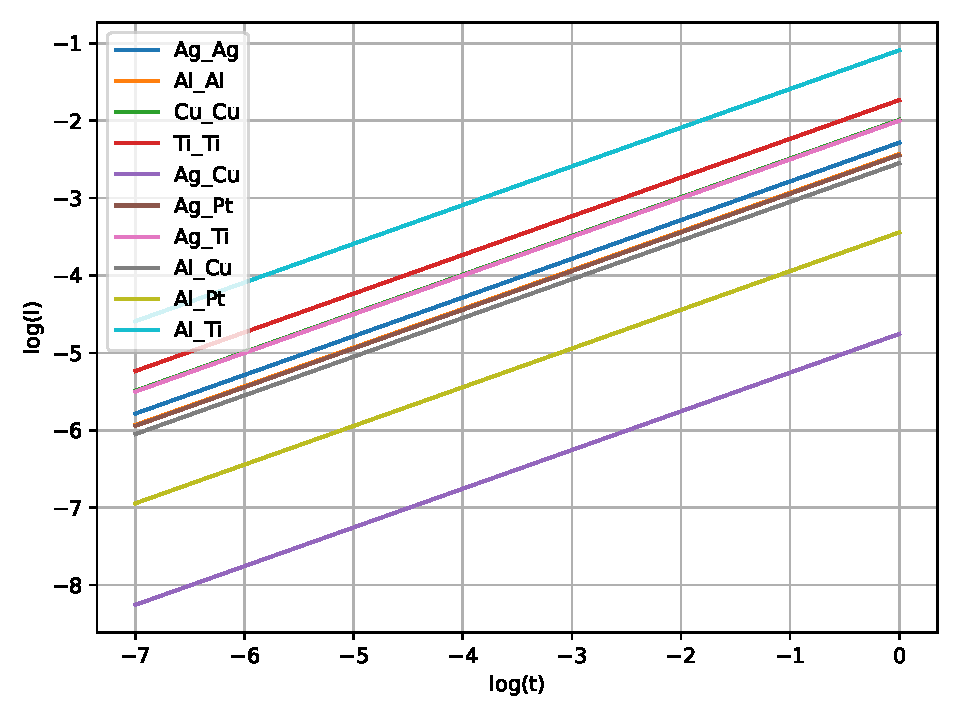
\includegraphics[width=0.5\textwidth]{graficas/log(l).pdf}}
 \caption{a) Diffusion distance $x$ (m) as a function of time $t$ (s) and b) logarithm of the diffusion distance $log(x)$ as a function of time $t$ ($s$). \\
 \textit{Source: Data from \citep{kakusan}, visualization by the author (code available at \citep{mygit}).}}
 \label{fig:diffusion}
\end{figure}


\subsection{Self-diffusion}

\begin{figure}[H]
 \centering
 \captionsetup{justification=centering}
  \subfloat[]{
   \label{fig:}
    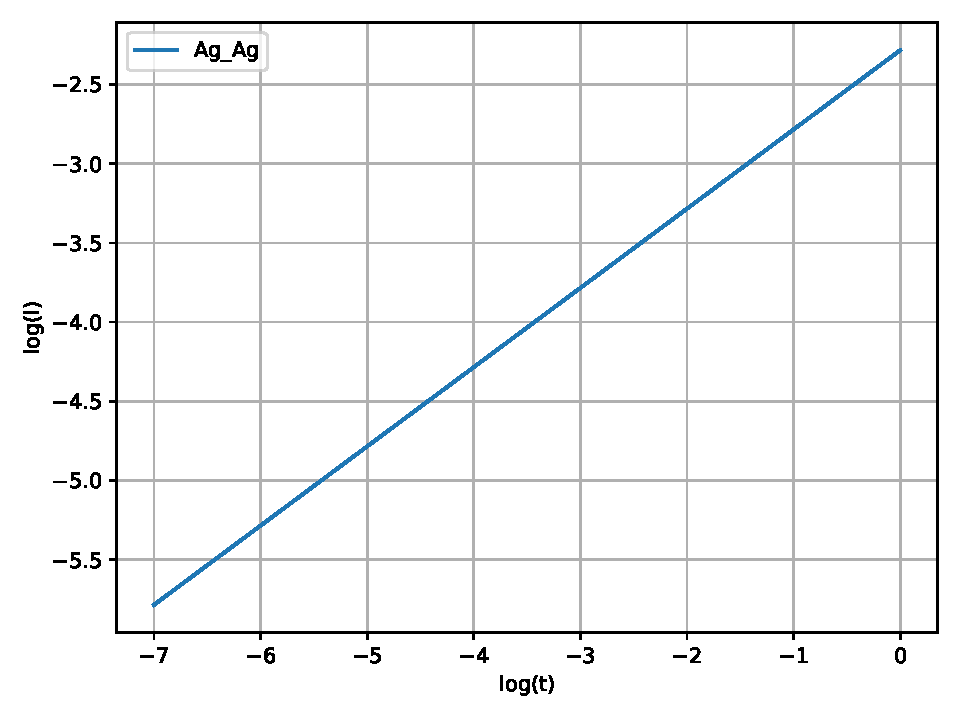
\includegraphics[width=0.5\textwidth]{graficas/Ag_Ag_log(l).pdf}}
  \subfloat[]{
   \label{fig:sigma4}
    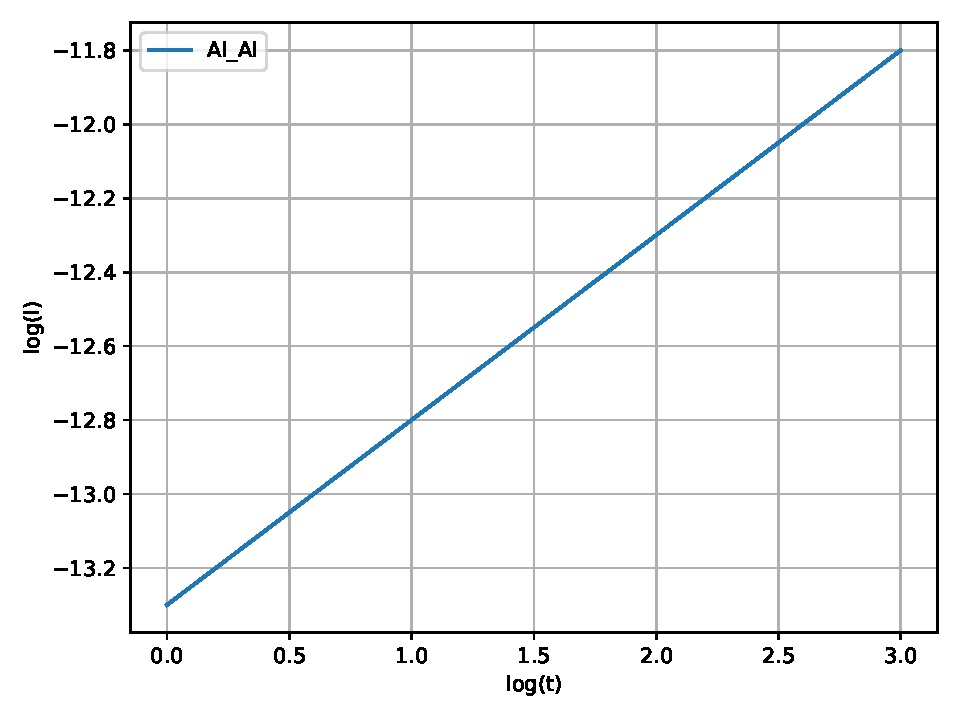
\includegraphics[width=0.5\textwidth]{graficas/Al_Al_log(l).pdf}} \\
  \subfloat[]{
   \label{fig:}
    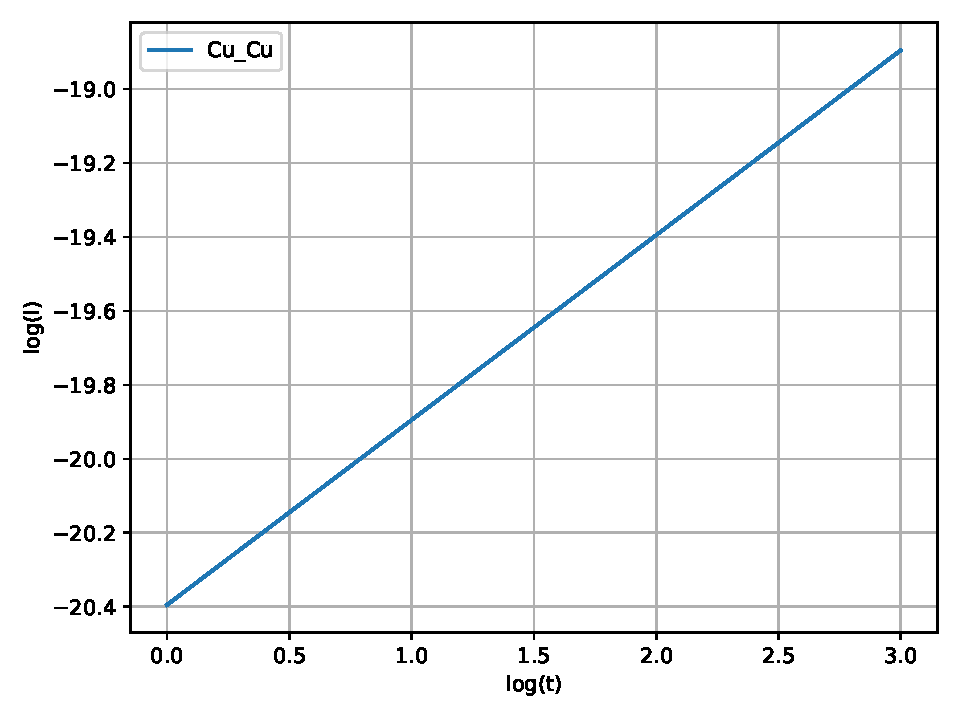
\includegraphics[width=0.5\textwidth]{graficas/Cu_Cu_log(l).pdf}}
  \subfloat[]{
   \label{fig:sigma4}
    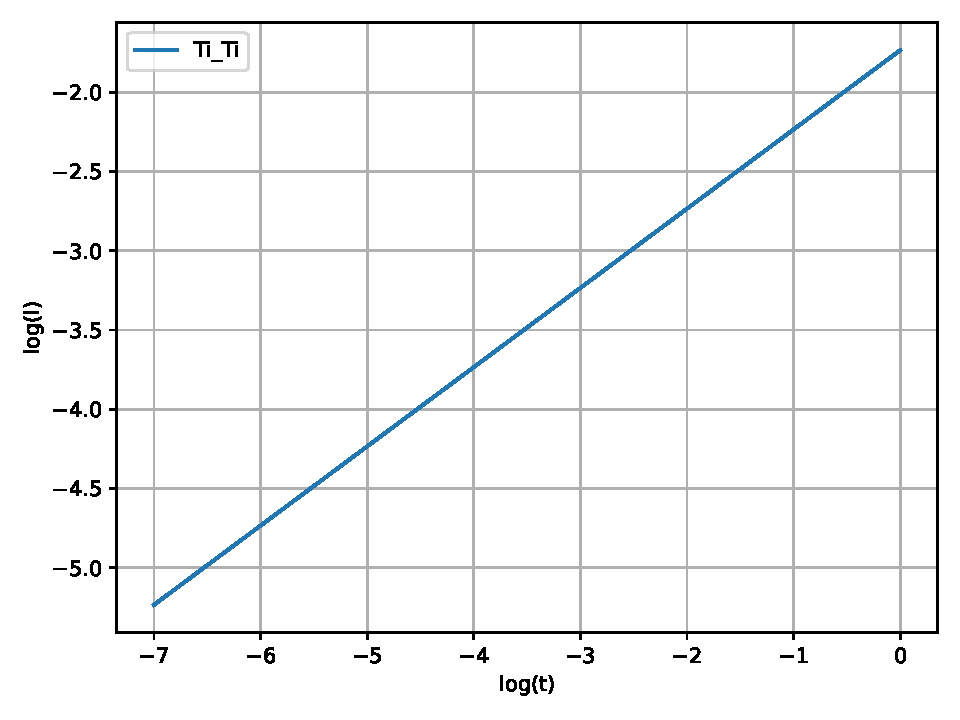
\includegraphics[width=0.5\textwidth]{graficas/Ti_Ti_log(l).pdf}}
 \caption{Distance of diffusion : a) silver, b) aluminum, c) copper and d) titanium.\\ 
 \textit{Source: Data from \citep{kakusan}, visualization by the author (code available at \citep{mygit}).}}
 \label{fig:selfdiff_lnd}
\end{figure}


\subsection{Solute diffusion}



(c) For the metals and solute atoms covered in question (a), assuming a sufficiently large sample size, graph the self-diffusion distance (logarithm) and the solute atom diffusion distance at room temperature against time (logarithm).
